\section{The Algorithms}
\label{sec:thealgorithm}
We are going to present a novel algorithm that extends our previous work
presented in~\cite{bkz05}. 
First we describe our previous work and in the following the new algorithm.
To the best of our knowledge this work is the first one that becomes possible
the construction of minimal perfect hash functions for sets in the order of 
billion of keys efficiently. 
And better, the generated functions are very compact and can be represented 
using approximately nine bits per key.

\subsection{A Main Memory Based Algorithm}

\subsection{An External Memory Based Algorithm}
The idea of behind the new algorithm is the traditional divide-to-conquer approach. 
The new algorithm consists of two steps that are presented in Fig.~\ref{fig:new-algo-main-steps}:
\begin{enumerate}
\item Using an universal hashing function~\cite{ss89} $h_1: S \to B$ the keys from $S$ are segmented to
a bucket set B, where $|B| = b$. We choice parameter $b$ in such way that any bucket will
contain more than 256 keys. 
This choice is crucial to make the new algorithm works and we give details about it hereinafter. 
\item The keys in each bucket are separetaly spread into a hash table.
\end{enumerate}
% For two-column wide figures use
\begin{figure}
% Use the relevant command to insert your figure file.
% For example, with the graphicx package use
\centering
  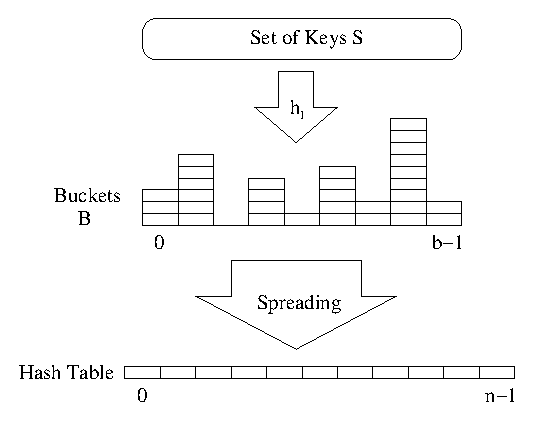
\includegraphics{figs/brz.ps}
% figure caption is below the figure
\caption{Main steps of the new algorithm.}
\label{fig:new-algo-main-steps}
\end{figure}

The main novelties are in the way the keys are segmented using external memory and spread using 
minimal perfect hash functions for each bucket. The next two sections describe each step in details.
\subsubsection{Segmentation}
\subsubsection{Spreading}
% Let us show how the minimal perfect hash function~$h$
% will be constructed.
% We make use of three auxiliary random functions~$h_1$, $h_2$ and~$h_3:U\to V$,
% where~$V=[0,t-1]$ for some suitably chosen integer~$t=cn$, where
% $n=|S|$.
% We build a random graph~$G=G(h_1,h_2)$ on~$V$,
% whose edge set is~$\big\{\{h_1(x),h_2(x)\}:x\in S\big\}$.
% There is an edge in~$G$ for each key in the set of keys~$S$.
% 
% In what follows, we shall be interested in the \textit{2-core} of
% the random graph~$G$, that is, the maximal subgraph of~$G$ with minimal
% degree at least~$2$
% (see, e.g., \cite{b01,jlr00}).
% Because of its importance in our context, we call the 2-core the
% \textit{critical} subgraph of~$G$ and denote it by~$G_\crit$.
% The vertices and edges in~$G_\crit$ are said to be \textit{critical}.
% We let~$V_\crit=V(G_\crit)$ and~$E_\crit=E(G_\crit)$.
% Moreover, we let~$V_\ncrit=V-V_\crit$ be the set of {\em non-critical}
% vertices in~$G$.
% We also let~$V_\scrit\subseteq V_\crit$ be the set of all critical
% vertices that have at least one non-critical vertex as a neighbour.
% Let $E_\ncrit=E(G)-E_\crit$ be the set of {\em non-critical} edges in~$G$.
% Finally, we let~$G_\ncrit=(V_\ncrit\cup V_\scrit,E_\ncrit)$ be the
% {\em non-critical} subgraph of~$G$.
% The non-critical subgraph $G_\ncrit$ corresponds to the ``acyclic part''
% of~$G$.
% We have $G=G_\crit\cup G_\ncrit$.
% 
% We then construct a suitable labelling $g:V\to\ZZ$ of the vertices
% of~$G$: we choose~$g(v)$ for each~$v\in V(G)$ in such
% a way that~$h(x)=g(h_1(x))+g(h_2(x))$ ($x\in S$) is a
% minimal perfect hash function for~$S$.
% We will see later on that this labelling~$g$ can be found in linear time
% if the number of edges in $G_\crit$ is at most $\frac{1}{2}|E(G)|$.
% 
% Figure~\ref{prog:mainsteps} presents a pseudo code for the algorithm.
% The procedure GenerateMPHF ($S$, $g$) receives as input the set of
% keys~$S$ and produces the labelling~$g$.
% The method uses a mapping, ordering and searching approach.
% We now describe each step.
% 
% \enlargethispage{\baselineskip}
% \enlargethispage{\baselineskip}
% \vspace{-11pt}
% \begin{figure}[htb]
% \begin{center}
% \begin{lstlisting}[
% ]
% procedure @GenerateMPHF@ (@$S$@, @$g$@)
%    Mapping (@$S$@, @$G$@);
%    Ordering (@$G$@, @$G_\crit$@, @$G_\ncrit$@);
%    Searching (@$G$@, @$G_\crit$@, @$G_\ncrit$@, @$g$@);
% \end{lstlisting}
%   \end{center}
% \vspace{-12pt}
%   \caption{Main steps of the algorithm for constructing a minimal
%            perfect hash function}
%   \vspace{-26pt}
%   \label{prog:mainsteps}
% \end{figure}
% 
% \subsection{Mapping Step}
% \label{sec:mapping}
% 
% The procedure Mapping ($S$, $G$) receives as input the set of keys~$S$ and
% generates the random graph $G=G(h_1,h_2)$, by generating two auxiliary
% functions~$h_1$, $h_2:U\to[0,t-1]$.
% 
% \def\tabela{\hbox{table}}
% %
% The functions~$h_1$ and~$h_2$ are constructed as follows.
% We impose some upper bound~$L$ on the lengths of the keys in~$S$.
% To define~$h_j$ ($j=1$,$2$), we generate an~$L\times\Sigma$ table
% of random integers~$\tabela_j$.
% For a key~$x\in S$ of length~$|x|\leq L$ and~$j\in\{1,2\}$, we let
% \begin{displaymath} \nonumber
% h_j(x) = \Big (\textstyle\sum_{i=1}^{|x|} \tabela_j[i, x[i]] \Big) \bmod t.
% \end{displaymath}
% The random graph~$G=G(h_1,h_2)$ has vertex set~$V=[0,t-1]$ and edge set
% $\big\{\{h_1(x),h_2(x)\}:x\in S\big\}$.  We need~$G$ to be
% simple, i.e.,
% $G$~should have neither loops nor multiple edges.
% A loop occurs when $h_1(x) = h_2(x)$ for some~$x\in S$.
% We solve this in an ad hoc manner: we simply let~$h_2(x)=(2h_1(x)+1)\bmod
% t$ in this case.
% If we still find a loop after this,
% we generate another pair $(h_1,h_2)$.
% When a multiple edge occurs we abort and generate a new pair~$(h_1,h_2)$.
% 
% \vspace{-10pt}
% \subsubsection{Analysis of the Mapping Step. }
% 
% We start by discussing some facts on random graphs.
% Let~$G=(V,E)$ with $|V|=t$ and $|E|=n$ be a random graph in the uniform
% model~$\cG(t,n)$, the model in which all the~${{t\choose2}\choose n}$ graphs
% on~$V$ with~$n$ edges are equiprobable.
% The study of~$\cG(t,n)$ goes back to the classical
% work of Erd\H os and R\'enyi~\cite{er59,er60,er61} (for a modern treatment,
% see~\cite{b01,jlr00}).
% Let $d=2n/t$ be the average degree of $G$.
% It is well known that, if~$d>1$, or, equivalently,
% if~$c<2$ (recall that we have $t=cn$),
% then, almost every~$G$
% contains\footnote{As is usual in the theory of random graphs, we use
% the terms `almost every' and `almost surely' to mean `with probability
% tending to~$1$ as~$t\to\infty$'.} a ``giant'' component of
% order~$(1+o(1))bt$, where~$b=1-T/d$, and~$0<T<1$ is the unique solution
% to the equation~$Te^{-T}=de^{-d}$.
% Moreover, all the other components of~$G$ have~$O(\log t)$ vertices.
% Also, the number of vertices in the 2-core of~$G$ (the maximal subgraph of $G$
% with minimal degree at least~$2$) that do not belong to the giant component
% is~$o(t)$ almost surely.
% 
% Pittel and Wormald~\cite{pw04} present detailed results
% for the 2-core of the giant component of the random graph~$G$.
% Since~$\tabela_j$ ($j\in\{1,2\}$) are random, $G=G(h_1,h_2)$~is a random
% graph.
% In what follows, we work under the hypothesis that~$G=G(h_1,h_2)$ is drawn
% from~$\cG(t,n)$.
% Thus, following~\cite{pw04}, the number of vertices of~$G_\crit$ is
% \begin{eqnarray} \label{eq:nvertices2core}
% |V(G_\crit)| = (1+o(1))(1-T)bt 
% \end{eqnarray}
% almost surely.  Moreover, the number of edges in this 2-core is
% \begin{eqnarray} \label{eq:nedges2core}
% |E(G_\crit)| = (1+o(1))\Big((1-T)b+b(d+T-2)/2\Big)t \\[-4mm]\nonumber
% \end{eqnarray}
% almost surely.
% Let~$d_\crit=2|E(G_\crit)|/|V(G_\crit)|$ be the average degree of~$G_\crit$.
% We are interested in the case in which~$d_\crit$ is a constant.
% 
% \enlargethispage{\baselineskip}
% \enlargethispage{\baselineskip}
% As mentioned before, for us to find
% the labelling $g:V\to\ZZ$ of the vertices of~$G=G(h_1,h_2)$ in linear time,
% we require that~$|E(G_\crit)|\leq\frac{1}{2}|E(G)|=\frac12|S|=n/2$.
% The crucial step now is to determine the value
% of~$c$ (in $t=cn$) to obtain a random graph $G=G_\crit\cup G_\ncrit$ with
% $|E(G_\crit)|\leq\frac{1}{2}|E(G)|$.
% 
% Table~\ref{tab:values} gives some values for~$|V(G_\crit)|$
% and~$|E(G_\crit)|$ using Eqs~(\ref{eq:nvertices2core})
% and~(\ref{eq:nedges2core}).
% The theoretical value for~$c$ is around~$1.152$, which is remarkably
% close to the empirical results presented in
% Table~\ref{tab:probability_cve1}.
% In this table, generated from real data, the probability $P_{|E(G_\crit)|}$
% that $|E(G_\crit)| \le \frac{1}{2}|E(G)|$ tends to~$0$ when $c < 1.15$ and it
% tends to $1$ when $c \ge 1.15$ and $n$ increases.  We found this match between
% the empirical and the theoretical results most pleasant,
% and this
% is why we consider that this random graph, conditioned on being simple,
% strongly resembles the random graph from the uniform model~$\cG(t,n)$.
% 
% 
% \vspace{-8pt}
% \begin{table}[!htb]
% {\footnotesize 
% \begin{center}
% \begin{tabular}{|c|c|c|c|c|c|}
% \hline
% $d$   & $T$  & $b$ & $|V(G_\crit)|$ & $|E(G_\crit)|$ & $c$ \\
% \hline
% %1.730 & 0.512 & 0.704 & 0.398$n$ & 0.496$n$ & 1.156 \\
% %1.732 & 0.511 & 0.705 & 0.398$n$ & 0.497$n$ & 1.155 \\
% %1.733 & 0.510 & 0.706 & 0.399$n$ & 0.498$n$ & 1.154 \\
% 1.734 & 0.510 & 0.706 & 0.399$n$ & 0.498$n$ & 1.153 \\
% 1.736 & 0.509 & 0.707 & 0.400$n$ & 0.500$n$ & 1.152 \\
% 1.738 & 0.508 & 0.708 & 0.401$n$ & 0.501$n$ & 1.151 \\
% 1.739 & 0.508 & 0.708 & 0.401$n$ & 0.501$n$ & 1.150 \\
% 1.740 & 0.507 & 0.709 & 0.401$n$ & 0.502$n$ & 1.149 \\
% %1.742 & 0.506 & 0.709 & 0.402$n$ & 0.503$n$ & 1.148 \\
% %1.744 & 0.505 & 0.710 & 0.403$n$ & 0.504$n$ & 1.147 \\
% %1.746 & 0.505 & 0.711 & 0.404$n$ & 0.506$n$ & 1.145 \\
% \hline
% \end{tabular}
% \end{center}
% \caption{Determining the $c$ value theoretically}
% \vspace{-42pt}
% \label{tab:values}
% }
% \end{table}
% 
% 
% \begin{table}
% {\footnotesize
% \begin{center}
% \begin{tabular}{|c|c|c|c|c|c|c|c|}
% \hline 
% \raisebox{-0.7em}{$c$} & \multicolumn{7}{c|}{\raisebox{-1mm}{URLs ($n$)}} \\
% \cline{2-8} 
%  & \raisebox{-1mm}{$10^3$} &\raisebox{-1mm}{$10^4$} &\raisebox{-1mm}{$10^5$} & \raisebox{-1mm}{$10^6$} & \raisebox{-1mm}{$2 \times 10^6$} & \raisebox{-1mm}{$3 \times 10^6$} & \raisebox{-1mm}{$4 \times 10^6$} \\
% \hline
% %1.10      & 0.01 & 0.00 & 0.00 & 0.00  & 0.00 & 0.00 & 0.00 \\
% %1.11      & 0.04 & 0.00 & 0.00 & 0.00  & 0.00 & 0.00 & 0.00 \\
% %1.12      & 0.12 & 0.00 & 0.00 & 0.00  & 0.00 & 0.00 & 0.00 \\
% 1.13      & 0.22 & 0.02 & 0.00 & 0.00  & 0.00 & 0.00 & 0.00 \\
% 1.14      & 0.35 & 0.15 & 0.00 & 0.00  & 0.00 & 0.00 & 0.00 \\
% 1.15      & 0.46 & 0.55 & 0.65 & 0.87  & 0.95 & 0.97 & 1.00 \\
% 1.16      & 0.67 & 0.90 & 1.00 & 1.00  & 1.00 & 1.00 & 1.00 \\
% 1.17      & 0.82 & 0.99 & 1.00 & 1.00  & 1.00 & 1.00 & 1.00 \\
% %1.18      & 0.91 & 0.97 & 0.98 & 1.00  & 1.00 & 1.00 & 1.00 \\
% %1.19      & 0.94 & 1.00 & 1.00 & 1.00  & 1.00 & 1.00 & 1.00 \\
% %1.20      & 0.98 & 1.00 & 1.00 & 1.00  & 1.00 & 1.00 & 1.00 \\[1mm]
% \hline
% \end{tabular}
% \end{center}
% \caption{Probability $P_{|E_\crit|}$ that $|E(G_\crit)| \le n/2$
% for different $c$ values and different number of keys for a collections of URLs}
% \vspace{-25pt}
% \label{tab:probability_cve1}
% }
% \end{table}
% 
% We now briefly argue that the expected number of iterations to obtain a simple
% graph~$G=G(h_1,h_2)$ is constant for $t=cn$ and $c=1.15$.  Let~$p$ be the
% probability of generating a random graph~$G$ without loops and without
% multiple edges. If~$p$ is bounded from below by some positive constant, then
% we are done, because the expected number of iterations to obtain such a graph
% is then~$1/p=O(1)$.  To estimate~$p$, we estimate the probability of
% obtaining~$n$ \textit{distinct} objects when we independently draw $n$~objects
% from a universe of cardinality~${t\choose2}={cn\choose2}\sim c^2n^2/2$, with
% replacement.  This latter probability is about~$e^{-{n\choose2}/{t\choose2}}$
% for large~$n$.  As~$e^{-{n\choose2}/{t\choose2}}\to e^{-1/c^2}>0$
% as~$n\to\infty$, the expected number of iterations is~$e^{1/c^2}=2.13$ (recall
% $c=1.15$).
% As the expected number of iterations is $O(1)$, the mapping step takes
% $O(n)$ time.
% 
% \vspace{-5pt}
% \subsection{Ordering Step}
% \label{sec:ordering}
% 
% The procedure Ordering ($G$, $G_\crit$, $G_\ncrit$) receives as
% input the graph~$G$ and partitions~$G$ into the two subgraphs
% $G_\crit$ and $G_\ncrit$, so that~$G=G_\crit\cup G_\ncrit$.
% For that, the procedure iteratively remove all vertices of degree 1 until done.
% 
% \enlargethispage{\baselineskip}
% Figure~\ref{fig:grafordering}(a) presents a sample graph with 9 vertices
% and 8 edges, where the degree of a vertex is shown besides each vertex.
% Applying the ordering step in this graph, the $5$-vertex graph showed in
% Figure~\ref{fig:grafordering}(b) is obtained.
% All vertices with degree 0 are non-critical vertices and the others are
% critical vertices. In order to determine the vertices in $V_\scrit$ we collect all vertices
% $v \in V(G_\crit)$ with at least one vertex $u$ that is in Adj$(v)$ and
% in $V(G_\ncrit)$, as the vertex 8 in Figure~\ref{fig:grafordering}(b).
% 
% \vspace{-5pt}
% \begin{figure*}[!htb]
% \begin{center}
% \scalebox{0.85}{\psfig{file=figs/grafordering.ps}}
% \end{center}
% \vspace{-10pt}
% \caption{Ordering step for a graph with 9 vertices and 8 edges}
% \vspace{-30pt}
% \label{fig:grafordering}
% \end{figure*}
% 
% 
% \subsubsection{Analysis of the Ordering Step. }
% 
% The time complexity of the ordering step is $O(|V(G)|)$ (see \cite{chm97}).
% As $|V(G)| = t = cn$, the ordering step takes $O(n)$ time.
% 
% \vspace{-5pt}
% \subsection{Searching Step}
% \label{sec:searching}
% 
% In the searching step, the key part is
% the {\em perfect assignment problem}: find $g:V(G)\to\ZZ$ such that
% the function $h:E(G)\to\ZZ$ defined by
% \begin{eqnarray}
%   \label{eq:phf}
%   h(e) = g(a)+g(b) \qquad(e=\{a,b\})
% \end{eqnarray}
% is a bijection from~$E(G)$ to~$[0,n-1]$ (recall~$n=|S|=|E(G)|$).
% We are interested in a labelling $g:V\to\ZZ$ of
% the vertices of the graph~$G=G(h_1,h_2)$ with
% the property that if~$x$ and~$y$ are keys in~$S$, then
% $g(h_1(x))+g(h_2(x))\neq g(h_1(y))+g(h_2(y))$; that is, if we associate
% to each edge the sum of the labels on its endpoints, then these values
% should be all distinct.
% Moreover, we require that all the sums $g(h_1(x))+g(h_2(x))$ ($x\in S$)
% fall between~$0$ and~$|E(G)|-1=n-1$, so that we have a bijection
% between~$S$ and~$[0,n-1]$.
% 
% The procedure Searching ($G$, $G_\crit$, $G_\ncrit$, $g$) receives
% as input~$G$, $G_\crit$, $G_\ncrit$ and finds a suitable
% $\log_2 |V(G)| + 1$ bit value for each vertex $v \in V(G)$, stored in the
% array~$g$.
% This step is first performed for the vertices in the
% critical subgraph~$G_\crit$ of $G$ (the 2-core of~$G$) and then it is
% performed for the vertices in $G_\ncrit$ (the non-critical subgraph
% of~$G$ that contains the ``acyclic part'' of $G$).
% The reason the assignment of the $g$~values is first
% performed on the vertices in~$G_\crit$ is to resolve reassignments
% as early as possible (such reassignments are consequences of the cycles
% in~$G_\crit$ and are depicted hereinafter).
% 
% \vspace{-8pt}
% \subsubsection{Assignment of Values to Critical Vertices. }
% \label{sec:assignmentcv}
% 
% The labels~$g(v)$ ($v\in V(G_\crit)$)
% are assigned in increasing order following a greedy
% strategy where the critical vertices~$v$ are considered one at a time,
% according to a breadth-first search on~$G_\crit$.
% If a candidate value~$x$ for~$g(v)$ is forbidden
% because setting~$g(v)=x$ would create two edges with the same sum,
% we try~$x+1$ for~$g(v)$. This fact is referred to as a {\em reassignment}.
% 
% \enlargethispage{\baselineskip}
% Let $A_E$ be the set of addresses assigned to edges in $E(G_\crit)$.
% Initially $A_E = \emptyset$.
% Let $x$ be a candidate value for $g(v)$.
% Initially $x = 0$.
% Considering the subgraph $G_\crit$ in Figure~\ref{fig:grafordering}(b),
% a step by step example of the assignment of values to vertices in $G_\crit$
% is presented in Figure~\ref{fig:searching}.
% Initially, a vertex $v$ is chosen, the assignment $g(v)=x$ is made
% and $x$ is set to $x + 1$.
% For example, suppose that vertex $8$ in Figure~\ref{fig:searching}(a) is
% chosen, the assignment $g(8)=0$ is made and $x$ is set to $1$.
% 
% \vspace{-12pt}
% \begin{figure*}[!htb]
% \begin{center}
% \scalebox{0.85}{\psfig{file=figs/grafsearching.ps}}
% \end{center}
% \vspace{-13pt}
% \caption{Example of the assignment of values to critical vertices}
% \vspace{-15pt}
% \label{fig:searching}
% \end{figure*}
% 
% In Figure~\ref{fig:searching}(b), following the adjacency list of vertex $8$,
% the unassigned vertex $0$ is reached.
% At this point, we collect in
% the temporary variable $Y$ all adjacencies of vertex $0$ that have been assigned
% an $x$ value, and $Y = \{8\}$.
% Next, for all $u \in Y$, we check if $g(u)+x \not \in A_E$.
% Since $g(8) + 1 = 1 \not \in A_E$, then $g(0)$ is set to $1$, $x$ is incremented
% by 1 (now $x=2$) and $A_E = A_E \cup \{1\}=\{1\}$.
% Next, vertex $3$ is reached, $g(3)$ is set to $2$,
% $x$ is set to $3$ and $A_E = A_E \cup \{2\}=\{1,2\}$.
% Next, vertex $4$ is reached and $Y=\{3, 8\}$.
% Since $g(3) + 3 = 5 \not \in A_E$ and $g(8) + 3 = 3 \not \in A_E$, then
% $g(4)$ is set to $3$, $x$ is set to $4$ and $A_E = A_E \cup \{3,5\} = \{1,2,3,5\}$.
% Finally, vertex $7$ is reached and $Y=\{0, 8\}$.
% Since $g(0) + 4 = 5 \in A_E$, $x$ is incremented by 1 and set to 5, as depicted in
% Figure~\ref{fig:searching}(c).
% Since $g(8) + 5 = 5 \in A_E$, $x$ is again incremented by 1 and set to 6,
% as depicted in Figure~\ref{fig:searching}(d).
% These two reassignments are indicated by the arrows in Figure~\ref{fig:searching}.
% Since $g(0) + 6 = 7 \not \in A_E$ and $g(8) + 6 = 6 \not \in A_E$, then
% $g(7)$ is set to $6$ and $A_E = A_E \cup \{6,7\} = \{1,2,3,5,6,7\}$.
% This finishes the algorithm.
% 
% \vspace{-15pt}
% \subsubsection{Assignment of Values to Non-Critical Vertices. }
% \label{sec:assignmentncv}
% 
% As $G_\ncrit$ is acyclic, we can impose the order in which addresses are
% associated with edges in $G_\ncrit$, making this step simple to solve
% by a standard depth first search algorithm.
% Therefore, in the assignment of values to vertices in $G_\ncrit$ we
% benefit from the unused addresses in the gaps left by the assignment of values
% to vertices in $G_\crit$.
% For that, we start the depth-first search from the vertices in $V_\scrit$
% because the $g$ values for these critical vertices have already been assigned
% and cannot be changed.
% 
% Considering the subgraph $G_\ncrit$ in Figure~\ref{fig:grafordering}(b),
% a step by step example of the assignment of values to vertices in
% $G_\ncrit$ is presented in Figure~\ref{fig:searchingncv}.
% Figure~\ref{fig:searchingncv}(a) presents the initial state of the
% algorithm.
% The critical vertex~$8$ is the only one that has non-critical 
% neighbours.
% In the example presented in Figure~\ref{fig:searching}, the addresses
% $\{0, 4\}$ were not used.
% So, taking the first unused address $0$ and the vertex $1$, which is
% reached from the vertex $8$, $g(1)$ is set to
% $0 - g(8) = 0$, as shown in Figure~\ref{fig:searchingncv}(b).
% The only vertex that is reached from vertex $1$ is vertex $2$, so
% taking the unused address $4$ we set $g(2)$ to $4 - g(1) = 4$,
% as shown in Figure~\ref{fig:searchingncv}(c).
% This process is repeated until the UnAssignedAddresses list becomes empty.
% 
% \vspace{-8pt}
% \begin{figure*}[!htb]
% \begin{center}
% \scalebox{0.85}{\psfig{file=figs/grafsearchingncv.ps}}
% \end{center}
% \vspace{-12pt}
% \caption{Example of the assignment of values to non-critical vertices}
% \vspace{-30pt}
% \label{fig:searchingncv}
% \end{figure*}
% 
% \subsubsection{Analysis of the Searching Step. }
% 
% We shall demonstrate that
% (i) the maximum value assigned to an edge is at most $n-1$ (that is, we
% generate a minimal perfect hash function), and
% (ii) the perfect assignment problem (determination of~$g$)
% can be solved in expected time $O(n)$ if the number of edges
% in $G_\crit$ is at most $\frac{1}{2}|E(G)|$.
% 
% \enlargethispage{\baselineskip}
% We focus on the analysis of the assignment of values to critical vertices
% because the assignment of values to non-critical vertices
% can be solved in linear time by a depth first search algorithm.
% 
% We now define certain complexity measures.
% Let $I(v)$ be the number of times a candidate value $x$ for
% $g(v)$ is incremented.
% Let $N_t$ be the total number of times that candidate values
% $x$ are incremented.
% Thus, we have~$N_t=\sum I(v)$, where the sum is over all~$v\in
% V(G_\crit)$.
% 
% For simplicity, we shall suppose that $G_\crit$, the 2-core of $G$, is
% connected.\footnote{The number of vertices in~$G_\crit$ outside the giant
%   component is provably very small for~$c=1.15$;
%   see~\cite{b01,jlr00,pw04}.} The fact that
% every edge is either a tree edge or a back edge (see, e.g., \cite{clrs01})
% then implies the following.
% 
% \begin{theorem} \label{th:nbedg}
% The number of back edges $N_\bedges$ of $G = G_\crit \cup G_\ncrit$
% is given by $N_\bedges = |E(G_\crit)| - |V(G_\crit)| + 1$.\qed
% \end{theorem}
% 
% \def\maxx{{\rm max}}
% Our next result concerns the maximal value $A_\maxx$ assigned to an edge $e
% \in E(G_\crit)$ after the assignment of $g$ values to critical vertices.
% 
% \begin{theorem} \label{th:Agrt}
%   We have $A_\maxx\le 2|V(G_\crit)| - 3 + 2N_{t}$.
% \end{theorem}
% \vspace{-15pt}
% 
% \enlargethispage{\baselineskip}
% \begin{proof}(Sketch)
% The assignment of $g$ values to critical vertices starts from 0,
% and each edge~$e$ receives the label $h(e)$
% as given by Eq.~(\ref{eq:phf}).
% The $g$ value for each vertex $v$ in $V(G_\crit)$ is assigned only once.
% A little thought shows that~$\max_v g(v)\leq |V(G_\crit)|-1+N_t$, where the
% maximum is taken over all vertices~$v$ in~$V(G_\crit)$.  Moreover, two
% distinct vertices get distinct~$g$ values.  Hence,
% $A_\maxx\le(|V(G_\crit)|-1+N_t)+(|V(G_\crit)|-2+N_t)
% \le2|V(G_\crit)|-3+2N_t$, as required.\qed
% \end{proof}
% 
% \vspace{-15pt}
% \subsubsection{Maximal Value Assigned to an Edge. }
% 
% In this section we present the following conjecture.
% \begin{conjecture} \label{conj:gretestaddr}
% For a random graph $G$ with $|E(G_\crit)|\leq n/2$ and
% $|V(G)| = 1.15n$,
% it is always possible to generate a minimal perfect hash function
% because the maximal value $A_\maxx$ assigned to an edge
% $e \in E(G_\crit)$ is at most $n - 1$.
% \end{conjecture}
% 
% Let us assume for the moment that $N_{t} \le N_\bedges$.
% Then, from Theorems~\ref{th:nbedg} and~\ref{th:Agrt},
% we have
% $A_\maxx\le2|V(G_\crit)|-3+2N_t\leq2|V(G_\crit)|-3+2N_\bedges
% \leq2|V(G_\crit)|-3+2(|E(G_\crit)|-|V(G_\crit)|+1)\le2|E(G_\crit)|-1$.
% As by hypothesis $|E(G_\crit)|\leq n/2$, we have
% $A_\maxx \le n - 1$, as required.
% 
% \textit{In the mathematical analysis of our algorithm, what is left
% open is a single problem:
% prove that $N_{t} \le N_\bedges$.}\footnote{%
%   Bollob\'as and Pikhurko~\cite{bp04} have investigated
% a very close vertex labelling problem for random graphs.
% However, their interest was on denser random graphs, and it seems that
% different methods will have to be used to attack the sparser case that
% we are interested in here.}
% 
% We now show experimental evidence that $N_{t} \le N_\bedges$.
% Considering Eqs~(\ref{eq:nvertices2core}) and~(\ref{eq:nedges2core}),
% the expected values for $|V(G_\crit)|$ and $|E(G_\crit)|$ for $c=1.15$ are
% $0.401 n$ and $0.501n$, respectively.
% From Theorem~\ref{th:nbedg},
% $N_\bedges = 0.501n - 0.401n + 1 = 0.1n + 1$.
% Table~\ref{tab:collisions1} presents the maximal value of $N_t$ obtained
% during 10,000 executions of the algorithm for different sizes of $S$.
% The maximal value of $N_t$ was always smaller than $N_\bedges = 0.1 n + 1$ and
% tends to $0.059n$ for $n\ge1{,}000{,}000$.
% 
% \vspace{-5pt}
% \begin{table}[!htb]
% {\footnotesize%\small
% \begin{center}
% \begin{tabular}{|c|c|}
% \hline
% $n$             & Maximal value of $N_t$\\
% \hline
% %$1{,}000$         & $0.091 n$ \\
% $10{,}000$        & $0.067 n$ \\
% $100{,}000$       & $0.061 n$ \\
% $1{,}000{,}000$     & $0.059 n$ \\
% $2{,}000{,}000$     & $0.059 n$ \\
% %$\vdots$        & $\vdots$ \\
% \hline
% \end{tabular}
% \end{center}
% }
% \caption{The maximal value of $N_t$ for different number of URLs}
% \vspace{-40pt}
% \label{tab:collisions1}
% \end{table}
% 
% \subsubsection{Time Complexity. }
% We now show that the time complexity of determining~$g(v)$
% for all critical vertices~$x\in V(G_\crit)$ is
% $O(|V(G_\crit)|)=O(n)$.
% For each unassigned vertex $v$, the adjacency list of $v$, which we
% call Adj($v$), must be traversed
% to collect the set $Y$ of adjacent vertices that have already been assigned a
% value.
% Then, for each vertex in $Y$, we check if the current candidate value $x$ is
% forbidden because setting $g(v)=x$ would create two edges with the same
% endpoint sum.
% Finally, the edge linking $v$ and $u$, for all $u \in Y$, is
% associated with
% the address that corresponds to the sum of its endpoints.
% Let $d_\crit=2|E(G_\crit)|/|V(G_\crit)|$ be the average degree of $G_\crit$,
% note that~$|Y|\leq|{\mathrm Adj}(v)|$, and suppose for simplicity
% that~$|{\mathrm Adj}(v)|=O(d_\crit)$.
% Then, putting all these together, we see that the time complexity of this
% procedure is
% \begin{eqnarray}
% &C(|V(G_\crit)|) = \sum_{v\in V(G_\crit)} \big[\:|{\mathrm Adj}(v)| +
% (I(v) \times|Y|) + |Y|\big]\nonumber\\
% &\qquad\qquad\qquad\leq\sum_{v\in V(G_\crit)}(2+I(v))|{\mathrm Adj}(v)|
% =4|E(G_\crit)|+O(N_t d_\crit).\nonumber
% \end{eqnarray}
% As $d_\crit=2\times0.501n/0.401n\simeq2.499$ (a constant) we have
% $O(|E(G_\crit)|)=O(|V(G_\crit)|)$.
% Supposing that $N_{t}\le N_\bedges$, we have, from Theorem~\ref{th:nbedg},
% that
% $
% N_{t}\le|E(G_\crit)|-|V(G_\crit)|+1
% =O(|E(G_\crit)|)$.
% We conclude that
% $C(|V(G_\crit)|)=O(|E(G_\crit)|) = O(|V(G_\crit)|)$.
% As $|V(G_\crit)| \le |V(G)|$ and $|V(G)| = cn$,
% the time required to determine~$g$ on the critical vertices is $O(n)$.
% \enlargethispage{\baselineskip}
% \vspace{-8pt}
